% How to use writeLaTeX: 
%
% You edit the source code here on the left, and the preview on the
% right shows you the result within a few seconds.
%
% Bookmark this page and share the URL with your co-authors. They can
% edit at the same time!
%
% You can upload figures, bibliographies, custom classes and
% styles using the files menu.
%
%%%%%%%%%%%%%%%%%%%%%%%%%%%%%%%%%%%%%%%%%%%%%%%%%%%%%%%%%%%%%%%%%%%%%%

\documentclass[12pt,english,brazil]{article}
\usepackage{sbc-template}
\usepackage{adjustbox}
\usepackage{graphicx,url}
\usepackage{graphics}
\usepackage{color}
\usepackage{colortbl}
\usepackage[utf8]{inputenc}  
% Coloquei esse pacote para tamanho pequeno de fonte
\usepackage{scalefnt}
\usepackage{multirow}
\usepackage{subfigure}
\usepackage{multicol}
\usepackage{babel}
\babeltags{br = brazil, en = english}
\usepackage[T1]{fontenc}
\usepackage{xspace}
\usepackage{url}
\usepackage{enumerate}

\usepackage{xargs}
\usepackage[colorinlistoftodos,prependcaption,textsize=tiny]{todonotes}
\newcommandx{\ups}[2][1=]{\todo[linecolor=red,backgroundcolor=red!25,bordercolor=red,#1]{\tiny Gerson: #2}\xspace}
\newcommandx{\aham}[2][1=]{\todo[linecolor=yellow,backgroundcolor=yellow!25,bordercolor=yellow,#1]{\tiny Gui: #2}\xspace}
     
\sloppy

\title{Estudo de viabilidade do uso de Raspberry como servidor R-Shiny}

\author{Guilherme de Souza\inst{1}, João Silveira\inst{1}, Giovani Jahn\inst{1}, \\Alfredo Goldman\inst{3}, Samuel Beskow$^4$, Gerson Geraldo H. Cavalheiro\inst{1}}

\address{PPGC ~~~~~~~~~~~~~~~~ $^4$PPCRH \\Universidade Federal de Pelotas (UFPel)\\
  Caixa Postal 354 -- 96010.610 -- Pelotas -- RS -- Brazil
\nextinstitute
Programa de Pós-Graduação em Hidrologia e Modelagem Hidrológica\\
\nextinstitute
  Instituto de Matemática e Estatística (IME) -- Universidade de São Paulo (USP)\\
  Rua do Matão, 1010 -- São Paulo -- SP -- Brazil
  \email{gdsdsilva@inf.ufpel.edu.br}
}

\begin{document} 

\maketitle
    
\en
\begin{abstract}
The use of servers is widespread in practically all computing areas. Notwithstanding this, the concern with the search for solutions aimed at reducing energy use is also a reality. In this article, we present the use of a Small Business Computer (SLC), the Raspberry Pi, as a low-cost alternative to provide application server services developed using the R language together with R-Shiny. To do so, a Raspberry Pi device was configured and compared, with an X86 architecture server. Scenarios and performance testing tools were applied and, through these, it was possible to evaluate and verify that the small board supports serving a low number of users without the use of any tuning techniques, thus confirming the veracity of the initially proposed premise.

\end{abstract}

\begin{resumo}
O uso de servidores esta difundido em praticamente todas as áreas computacionais. Não obstante a isso, a preocupação com a busca de soluções atentas à redução do uso de energia, também é uma realidade.  Apresentamos neste artigo o uso de uma Small Business Computer (SLC), a Raspberry Pi, como uma alternativa de baixo custo para prover serviços de servidor de aplicação desenvolvida utilizando a linguagem R juntamente com R-Shiny. Para tal, um dispositivo Raspberry Pi foi configurado e confrontado quanto ao seu desempenho, com um servidor de arquitetura X86. Cenários e ferramentas de testes de desempenho foram aplicados e, por meio destes, pôde-se avaliar e constatar que a small board consegue atender um baixo número de usuários sem a utilização de quaisquer técnica de tuning, assim, confirmando a veracidade da premissa inicialmente proposta.


\end{resumo}



\section{Introdução}

A  decisão por realizar, ou não, um investimento financeiro passa, muitas vezes, pela análise de uma grande
massa de dados. Os setores agrícolas e de obras civis possuem situações onde esta análise tem relevada importância, considerando aspectos hidrológicos. No contexto da agricultura, a decisão
por uma cultura, pelo agricultor, ou pela taxa de juros a ser aplicada, por uma entidade voltada ao
financiamento rural, depende da análise, entre outros, dos regimes hídricos do local onde a plantação ou
a aplicação dos recursos será realizada. A análise dos regimes hídricos dependem de decisões sobre implantação de infraestruturas civis, como pontes, barragens para reservatórios aquíferos
ou geração de energia e mesmo para dimensionamento de telhados de imóveis. A pura visualização de grande massas dados, por si, é complexa. Torna-se ainda mais complexa quando a visualização depende do tratamento dos dados segundo modelos que regem a análise do problema a ser considerado.

Para atender a necessidade de análise da grande massa de dados associadas aos aspectos hídricos, foi desenvolvida a aplicação WebSYHDA \cite{syhda}. O WebSYHDA é uma ferramenta, disponibilizada na Web, para aplicação de modelos hídricos e apresentação de gráficos com o resultado destes. A
ferramenta oferece um conjunto de recursos que permite a aplicação de diferentes modelos hídricos sobre
séries temporais registrando dados de rios, vazão e índices de precipitação. O WebSYHDA
foi desenvolvido em R, com apoio do pacote de visualização Shiny. Implantado em um servidor R, essa
ferramenta foi projetada para atender diferentes usuários simultaneamente.

Enquanto um serviço R, o suporte de operação do WebSYHDA é realizado de forma convencional pelo servidor Shinyapps.io\footnote{Shinyapps.io: \url{https://www.shinyapps.io/}} . Nessa etapa do trabalho busca-se avaliar as necessidades de
estrutura física para viabilizar esse serviço. O presente artigo avalia a escalabilidade em termos de número
de usuários WebSYHDA ativos simultaneamente em dois modelos de arquitetura: um servidor convencional
e um dispositivo de borda (\emph{small board}). 
No contexto do trabalho realizado, as métricas de desempenho, que são valores brutos que provem a base para alguma forma de pesquisa ou estudo e podem ser compostos por valores de diversas categorias e formato. Tem assim por finalidade quantificar objetivamente as funções de coletas de dados de avaliação e desempenho.
O caso de estudo encaminhado considera o serviço WebSYHDA, desenvolvido com a finalidade de processamento complexo de séries hidrológicas. São consideradas duas plataformas de suporte: um servidor com arquitetura convencional e um dispositivo de baixa capacidade (\emph{small board}). 
%O objetivo deste estudo é identificar componentes do software, atualmente construído de forma monolítica, na forma de microserviços.

O presente artigo está organizado da seguinte forma: na Seção~\ref{sec:TrabalhosRelacionados} serão apresentados trabalhos relacionados, na Seção~\ref{sec:WebSYHDA} é apresentada a aplicação utilizada como \emph{benchmark}. A Seção~\ref{sec:metodologia} são apresentadas as ferramentas utilizadas para realização dos experimentos. Na Seção~\ref{sec:Resultados}, são descritos os resultados obtidos considerando os cenários representativos. As considerações finais e trabalhos futuros se encontram na Seção~\ref{sec:conlusao}.

\section{Trabalhos Relacionados} \label{sec:TrabalhosRelacionados}

O estudo da escalabilidade de servidores no atendimento aos usuários é constante na literatura \cite{generic1}, \cite{generic5}, \cite{generic3}, \cite{generic4}. Nos últimos anos, esse estudo passou a incluir a análise das questões
energéticas \cite{generic6}, \cite{generic7}, \cite{generic8}. Neste contexto, o uso de dispositivos de borda, os chamados \emph{small
boards}, em substituição a servidores convencionais tem se apresentado como alternativa.

Inicialmente, com um propósito similar ao WebSYHDA, no que tange ao uso de R e a estrutura Shiny, cita-se o  trabalho de \cite{CIPR} que utiliza os referidos recursos para criar uma aplicação web denominada \emph{Cluster Identity PRedictor}\footnote{Cluster Identity PRedictor: \url{https://github.com/atakanekiz/CIPR-Package}} (CIPR), que fornece uma interface gráfica de usuário para pontuar perfis de expressão gênica de \emph{clusters} de células.
Em outro contexto, com a finalidade de criar um servidor de arquivos utilizando um Raspberry Pi, para guardar os dados e poder compartilhar na rede. Assim, concluiu-se que o dispositivo pode ser utilizado com o propósito em questão, com economia de custos sem, contudo, deixar de ser viável para esta aplicação, observando-se apenas algumas variações de desempenho dependendo do tipo de armazenamento \cite{bruschi2016teste}.

A Raspberry Pi também foi utilizado para propor a viabilidade de sua utilização em hospedar um \emph{honeypot}, mostrando que sua efetividade irá depender da eficiência do \emph{software} utilizado e também do tamanho e complexidade da rede em que ficará esse dispositivo, para dar efetividade ao objetivo proposto \cite{honeypot}. Também dentro desse contexto de propor funcionalidades "servers" ao Raspberry Pi \cite{inproceedings}, outrora já mostrara que o uso de um computador de baixo custo - a Raspberry Pi, pode ser usado de forma segura como um servidor web,  propiciando economia de energia.

Em \cite{Joao} propôs avaliar a substituição do hardware convencional por um hardware de baixo consumo que respeite o \emph{Service-Level-Agreement} (SLA) e reduza o consumo de energia dos \emph{data centers}, assim tornando viável o uso de uma em uma nuvem computacional. A proposta incluiu a implementação de um Raspbarry Pi B+ como um nodo computacional de baixo consumo energético. Para tal, adaptações na arquitetura e no \emph{hipervisor} se fizeram necessárias.

Para a elaboração deste compendio, os testes e medições foram realizados executando o \emph{bechmark YCSB Yahoo! Cloud Serving Benchmark}, um sistema de código aberto e conjunto de programas para avaliar as capacidades de recuperação e manutenção de programas de computador. É frequentemente usado para comparar o desempenho relativo dos sistemas de gerenciamento de banco de dados NoSQL e nuvens. Com a análise das vazões das operações realizadas, pode-se perceber um gargalo de processamento quando comparado ao nó de um dispositivo de baixo consumo. Contudo, a implementação do Raspberry Pi B+ em uma nuvem, ainda sim é vantajosa.

Em \cite{PiConsumo} é evidenciada a mesma preocupação com o alto consumo de energia proveniente de ambientes vindo das \emph{clouds}. Ainda assim, até 2012, 10,82\% da população contribui com 0,03\% da energia consumida mundialmente, com o uso de 770 milhões de \emph{gateways} e \emph{routers} domésticos. Levando em consideração que os maiores consumos ocorrem por parte de máquinas com um \emph{hardware} mais poderoso, ainda sim não se pode ignorar o consumo vindo por parte de tais dispositivos, pois 43\% dos mesmos se mantém ligados diariamente, ociosos em boa parte do tempo, onde poderiam vir a desempenhar funções de pré-carregamento para usuário (ou seja, armazenamento em cache, pré-busca de conteúdo, execução de serviços locais). A Raspberry Pi vem sendo utilizada para inúmeras aplicações no qual fomenta o uso de tais aplicações com a visão em baixo consumo energético. \cite{PiConsumo}, apresenta o PowerPi um modelo de  potência concentrando-se no consumo de energia da Raspberry Pi a fim de derivar novas possíveis estratégias de consumo de energia.

Com os estudos aqui apresentados, observa-se a importância de explorar os dispositivos de baixa capacidade a fim de obter resultados qualitativos/quantitativos de seu desempenho. Porém não se discute aplicativos R-Shiny, dada a sua execução não nativa em dispositivos ARM. Assim o estudo de caso documentado neste artigo, é considerada uma aplicação desenvolvida sob um servidor R-Shiny.
%No estudo de caso documento neste artigo, é considerada uma aplicação desenvolvida sob um servidor R, onde o mesmo deve possuir algumas adaptações disponíveis em documentações para execução em dispositivos de arquitetura ARM. 


\section{WebSYHDA}\label{sec:WebSYHDA}

Engenharia e gestão de recursos hídricos mantém uma grande dependência de séries hidrológicas. No entanto, o processamento destas séries é complexo, geralmente dependente de métodos numéricos para resolução, e é suscetível a erros quando feito de forma manual. Esses aspectos frequentemente dificultam a elaboração de projetos que depende da análise e estudo de séries hidrológicas. Com isso O Grupo de Pesquisa em Hidrologia e Modelagem Hidrológica em Bacias Hidrográficas/CNPq da UFPEL, propôs, desenvolveu e mantem O \emph{System of Hydrological Data Acquisition and Analysis} ou SYHDA \cite{syhda}.

A plataforma recentemente passou por uma migração para o modelo Web, onde encontra-se em constante desenvolvimento. É integralmente desenvolvida em R, com auxílio do RStudio e de inúmeras bibliotecas gratuitas de uso geral, uso específico para a hidrologia e de funcionalidades para ambiente Web. %li no cobalto

O WebSYHDA permite a importação de dados do Hidroweb/ANA\footnote{ANA: \url{https://dadosabertos.ana.gov.br}}, para dados de vazão, chuva e nível. Estes dados são reconhecidos pela plataforma de forma automática. Outras fontes de dados estão sendo implementadas na plataforma, como BDMEP/INMET\footnote{INMET: \url{https://portal.inmet.gov.br}} e dados oriundos de estações de monitoramento diversas com formatos definidos pelo usuário.

% adicionei uma parte (joão)
A plataforma em sua versão atual, conta com diversas funcionalidades, bem como: constituição de séries históricas em diferentes intervalos de tempo, estatísticas descritivas, representações gráficas, testes não paramétricos, consistência de dados de chuva, análise de frequência local e análise de frequência regional. Os resultados são estruturados de forma dinâmica, assim permitindo o manuseio pelo usuário final, permitindo ainda a possibilidade de exportação e salvar o estado atual do projeto. 

\subsection{Linguagem R} \label{sec:R}

R é uma linguagem e ambiente com foco em computação estatística e gráficos. Assim, R permite desenvolver e publicar gráficos bem projetados \cite{whatR}, semelhantemente a C/C++ e outras linguagens disponíveis no mercado, R também permite o desenvolvimento por meio de módulos, mas ainda se tratando de uma única e grande aplicação. Desta forma, aplicações R são executadas em \emph{thread} único, não sendo possível o atendimento de dois, ou mais, usuários simultaneamente. Para as aplicações em que os cálculos possuem baixa granularidade, na ordem de poucas dezenas ou centenas de milissegundos, o fato da aplicação ser \emph{mono-thread} não gera grande impacto na experiência do usuário: um único processo R  pode atender de 5 a 30 solicitações por segundo \cite{ShinyappsEscalabilidade}. 

Entre tanto, para uma aplicação como o WebSYHDA e outras, onde a simultaneidade entre usuários podem ocorrer de forma frequente, acaba por resultar em respostas demoradas para os demais usuários, dado a dependência do tempo de processamento para o cálculo que estiver em execução. A fim de melhorar o desempenho para compensar o número de usuários, o escalonamento de hardware pode ser feito, porém o emprego de \emph{hardware} para suporte pode ser empregado de forma pouco eficiente dado a configuração de balanceamento permitida. %De mesma maneira ocorre se houver o uso insuficiente, onde o custo por hardware ocioso deixa a desejar.

\subsection{Shiny} \label{sec:Shiny}

Para o desenvolvimento de aplicativos \emph{web} fazendo uso da linguagem R, a RStudio mantém o pacote \emph{Shiny}\footnote{Shiny: \url{https://shiny.rstudio.com}}. Este pacote R que facilita a construção de aplicativos interativos. Permitindo hospedar aplicativos independentes em uma página da \emph{web} ou incorporá-los em documentos R \email{Markdown} ou construir painéis. 

Assim, torna-se possivel apresentar gráficos dinâmicos e interativos por meio de pacotes como, ggvis\footnote{ggvis: \url{https://ggvis.rstudio.com/}}, ggiraph\footnote{ggiraph: \url{https://davidgohel.github.io/ggiraph}}, plotly\footnote{plotly: \url{https://plotly.com/}} entre outros mantidos pela RStudio ou pela comunidade. Permitindo ainda, estender os aplicativos \emph{Shiny} com temas CSS (\emph{Cascading Style Sheets}), \emph{htmlwidgets} e ações JS (\emph{JavaScript}).


\section{Metodologia} \label{sec:metodologia}

Visto que a demanda de serviços \textit{web} ocupa a maior parte das aplicações na nuvem, maiores são os esforços para otimização das aplicações para um menor consumo de requisitos e rede, mantendo, no entanto, níveis de desempenho aceitáveis aos usuários. Neste trabalho o aspecto tratado é o dimensionamento das necessidades de \emph{hardware} para atender a demanda de processamento do WebSYHDA. O estudo de caso avalia o desempenho obtido com uma arquitetura padrão x86 convencional com uma \emph{small board} modelo Raspberry Pi 3. O objetivo do estudo é, considerando a natureza sequencial de atendimento às solicitações, determinar se este \emph{smallboard} apresenta a mesma eficiência de atendimento a uma aplicação real, o WebSYHDA, que a já observada em trabalhos anteriores  \cite{silva2019estudo}.

O procedimento de avaliação empregou a exploração do servidor R nas duas arquiteturas. A carga de trabalho ao qual estes servidores responderam correspondeu a demanda gerada por traços obtidos de consultas reais. A carga foi submetida aos respectivos servidores pela  ferramenta \emph{Shinycannon}, permitindo quantificar o número de usuários suportados e latência do aplicativo.


\subsection{Shinycannon} \label{sec:Shinycannon}

\textit{Shinycannon}\footnote{Shinycannon: \url{https://github.com/rstudio/shinycannon}} é uma ferramenta de linha de comando que possibilita testes de carga em aplicativos R. Assim, permitindo aos desenvolvedores analisarem a escalabilidade de seu aplicativo simulando um número variável de usuários simultaneos.

A ferramenta acompanha o pacote \textit{shinyloadtest}\footnote{Shinyloadtest: \url{https://rstudio.github.io/shinyloadtest}}, mantido pela própria RStudio. O pacote é responsável por gerar uma gravação de uma sessão real de usuário, a qual deve representar o uso típico do serviço a ser avaliado \cite{shinyloadtest} e a qual servirá como base para o estudo do comportamento. A partir desta sessão gravada, durante um intervalo de tempo parametrizado, diversos usuários podem ser simulados executando o mesmo conjunto de operações. Como resultado da simulação de operação, são oferecidos diferentes informações sobre o atendimento do serviço, como tempos de utilização de CPU e de espera do usuário por respostas.

\subsection{Hardware}\label{sec:Hardware}
Com a popularização do uso de serviços providos pela computação em nuvem, o consumo energético dos \emph{data centers} também aumentou, chegando a 270 TWh em 2012 \cite{VanHeddeghem:2014:TWI:2657027.2657141}, estimando chegar a mais de 2\% do consumo da energia mundial após 2020 \cite{energy}. Buscando alternativas de evitar esse alto consumo energético das máquinas convencionais utilizadas em \emph{data centers}, o uso de dispositivos com arquitetura ARM, que possuem baixo consumo energético, são uma das estratégias possíveis.

Neste trabalho, é analisado a capacidade de resposta de um Raspberry Pi 3 no atendimento aos serviços providos pelo WebSYHDA com o oferecido por uma arquitetura x86 convencional. As características destes dois equipamentos são apresentadas na Tabela \ref{tab:specs}. 

\begin{table}[h]
\centering
\caption{Especificação de \textit{hardware} dos dispositivos}
\begin{tabular}{c|c|c}
\hline
\textbf{Especificação}            & \textbf{x86} & \multicolumn{1}{l}{\textbf{Raspberry PI3}} \\ \hline
\textbf{Processador} &
  \begin{tabular}[c]{@{}c@{}}Intel(R) Xeon(R) CPU \\ E3-1220 v3 @ 3.10GHz\end{tabular} &
  \begin{tabular}[c]{@{}c@{}}BCM2837 64bit \\ Quad Core 1.2GHz\end{tabular} \\ \hline
\textbf{Arquitetura}              & x86                 & ARMv8                                      \\ \hline
\textbf{RAM}                      & 8GB                 & 1GB                                        \\ \hline
\textbf{Armazenamento}            & HD                  & Micro SD                                   \\ \hline
\textbf{Máxima corrente / Tensão} & 16A/+12V1           & 2.4A/5V                                    \\ \hline
\end{tabular}
\label{tab:specs}
\end{table}
    
Para comparativo de desempenho, utilizou-se um dispositivo de arquitetura x86.
O \textit{server} selecionado para tal comparativo, tem suas especificações apresentadas na Tabela ~\ref{tab:specs}, informações obtidas pelo comando \textit{dmidecode}, o qual apresenta todas informações disponíveis sobre o dispositivo, possibilitando uma pesquisa mais especifica dentro dele atribuindo ao comando \textit{dmidecode --type} concatenado com uma chave da tabela de representação do comando, como a chave quatro, nos demonstrará todas especificações do processador e assim por diante.

\subsection{Metodologia dos Testes}\label{sec:MetodologiaDosTestes}
A fim de testar o aplicativo no seu estágio atual de desenvolvimento e também encontrar cargas próximas ao limite da Raspberry PI3, consideramos a documentação como base, onde a mesma demonstra qual seria aproximadamente o limite de tempo de resposta do aplicativo dada a quantidade de usuários \cite{documentShiny}.

%Em um primeiro momento, analisamos o uso mais comum do sw, ou seja, seu uso diário por engenheiros hídricos, a Figura ~\ref{usoWebSYHDA} demonstra o conjunto de ações tomada dentro do aplicativo. Com isso utilizamos o pacote \emph{shinyloadtest}, assim permitindo a gravação deste conjunto de passos. 
Em um primeiro momento, buscou-se um teste que fosse característico de um fluxo típico de um usuário, fazendo uso de várias técnicas empregadas em diversas análises hidrológicas, porém com foco em tarefas que requerem maior processamento. Optou-se por utilizar o módulo de Análise de Frequência Regional para o teste, visto que o mesmo atende ao critério de uso anterior, assim como a exigência de múltiplos arquivos para computar os resultados. A Figura ~\ref{usoWebSYHDA} ilustra o conjunto de ações tomada para execução do teste dentro do aplicativo, sendo estas:

%A Figura ~\ref{usoWebSYHDA} ilustra o conjunto de ações tomada dentro do aplicativo. Com isso utilizamos o pacote \emph{shinyloadtest}, assim permitindo a gravação deste conjunto de passos. 

% descrição dos passos da Figura 2 (joão)
\begin{enumerate}[i.]
  \item Importar arquivos. A primeira etapa consistem em importar, para o servidor, um total de 10 arquivos do Hidroweb\footnote{Hidroweb: \url{https://www.snirh.gov.br/hidroweb}}, contendo dados de vazão da região a ser analisada.
  \item Aplicar o limiar de falhas de 31 dias, eliminando da série anual os anos onde há mais de 31 falhas (dias sem medição).
  \item Constituir séries anuais. Selecionar o período anual para transformar as séries diárias em anuais.
  \item Selecionar arquivos importados. No módulo de Análise de Frequência Regional  é possível selecionar, dentre os arquivos importados, quais serão utilizados na análise. No estudo realizado foram selecionados todos os 10 arquivos.
  \item Análise de frequência regional. Aplicação do modelo. A partir dos dados, são computados os Momentos-L de cada série anual, as medidas de heterogeneidade da região e a sua função regional.
  \item Visualização. Tabelas e gráficos representando os resultados da aplicação do modelo são gerados.
\end{enumerate}

\begin{figure}[htbp]
  \centering 
  \includegraphics[scale=.4]{paperWSCAD2021/figures/useWebSYHDADrawio-horizontal.png}
  \caption{Exemplo dos passos seguidos pelo usuário}
  \label{usoWebSYHDA}
\end{figure}

Uma aferição inicial mostrou que o tempo de atendimento a uma sessão de usuário, realizando as operações registradas pelo \emph{shinyloadtest}, é atendido e inferior a dois minutos no servidor implantado na Raspberry. Este tempo representa o tempo de execução tendo o servidor inteiramente dedicado ao usuário. O procedimento de coleta de dados de desempenho considerou a escalabilidade do atendimento ao serviço, coletando dados de desempenho com 1, 10 e 20 usuários simultâneos no \emph{server} e 1, 2, 3 e 4 usuários simultâneos na Raspberry, submetendo o mesmo conjunto de operações, dentro de uma janela de, também, dois minutos.


%Nesses passos 10 arquivos foram utilizandos ... onde realiza ....

O limite de usuários, 20 no server e 4 na Raspberry, foi determinado em função da configuração padrão do servidor R sobre o \emph{hardware} disponível. Acima deste número de usuários é devolvido um código de erro informando a inviabilidade de atendimento. Todo o roteiro de testes e os arquivos gerados aqui apresentados, estão disponíveis no GitHub\footnote{GitHub: \url{https://github.com/SouzaGuilherme/research_PI3_R-Shiny-server}}.

\section{Resultados} \label{sec:Resultados}

A análise dos resultados do experimento é focado na avaliação do uso dos recursos de \emph{hardware} disponível durante o período de tempo em que o número total de usuários simultâneos se encontra ativo. Os gráficos desta seção representam os diferentes estados das sessões executadas pelos diferentes usuários ativos. Nestes gráficos, as linhas representam as sessões e, no plano horizontal, a passagem do tempo. O período de tempo que interessa a análise é aquele a partir do instante de tempo 0~s, representando o momento em que todos os usuários simultâneos encontram-se ativos. Nas execuções com um usuário, a segunda linha pontilhada marca o tempo em que o processamento das solicitações deste único usuário foi concluído. Quando da execução de mais de um usuário, a segunda linha pontilhada, marca o limite do período de 2 minutos (120~s) em que é realizada a análise. 

Em um primeiro momento observamos a execução com somente um usuário ativo em ambas arquiteturas, Figura~\ref{fig:x64}.a e Figura~\ref{fig:PI3}.a. É possível observar que, em ambos casos, a taxa de ociosidade dos processadores, representado pela cor cinza, é significativa. Este aspecto caracteriza disponibilidade de processamento e, portanto possibilidade de atendimento a um maior número de usuários simultâneos. 

Nos experimentos com 10 e 20 usuários simultâneos na arquitetura x86, Figuras~\ref{fig:x64}.b e \ref{fig:x64}.c, os dados de resultado revelaram aproveitamento do tempo ocioso no atendimento ao maior número de usuários simultâneos. Em relação ao tempo total de atendimento a cada usuário, o tempo limite de 2 minutos não foi ultrapassado.

Na Raspberry Pi 3, dada as suas características de \emph{hardware}, o limite no número de usuários simultâneos é 4. O comportamento da execução está registrado na Figura~\ref{fig:PI3}. Comparando os dados destes traços de execução com os oferecidos pela arquitetura x86, observa-se que seu \emph{hardware} não permite aproveitamento eficiente dos tempos de ociosidade. Também verifica-se aumento no tempo total para conclusão das requisições, a despeito da diferença de escala nos gráficos gerados pela ferramenta.

\begin{figure}[htbp]
  \centering 
  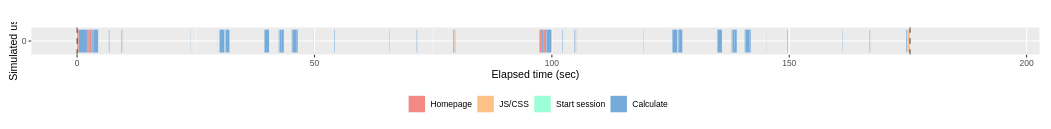
\includegraphics[scale=.4]{paperWSCAD2021/figures/user_x64_1_worker.png}\\(a) 1 usuário
    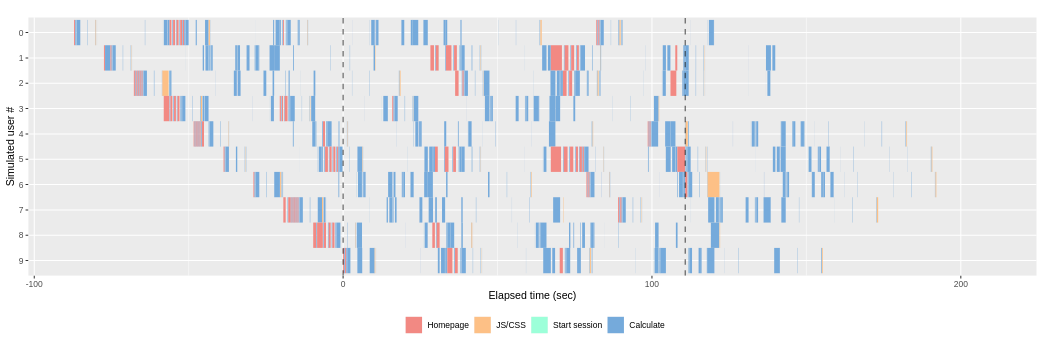
\includegraphics[scale=.4]{paperWSCAD2021/figures/user_x64_10_worker.png}\\(b) 10 usuários
  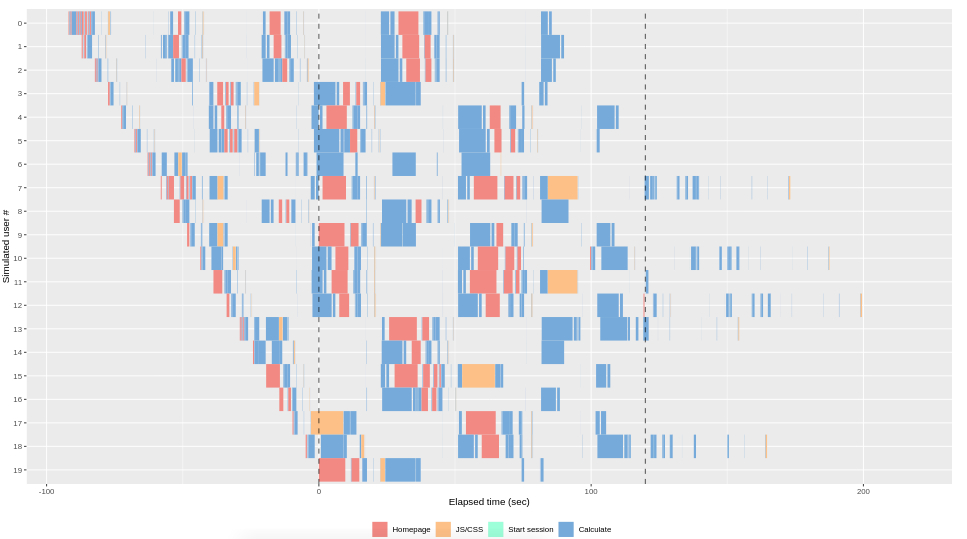
\includegraphics[scale=.4]{paperWSCAD2021/figures/user_x64_20_worker.jpg}\\(c) 20 usuários
\caption{Traço de execução do simulador no servidor x86.}
  \label{fig:x64}
\end{figure}


\begin{figure}[htbp]
  \centering 
  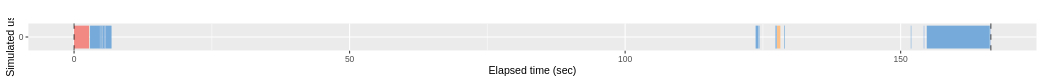
\includegraphics[scale=.4]{paperWSCAD2021/figures/user_PI3_1_worker_edit.jpg}\\(a) 1 usuário
 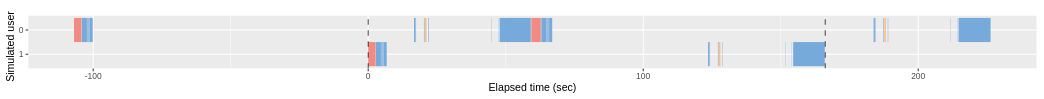
\includegraphics[scale=.4]{paperWSCAD2021/figures/user_PI3_2_worker_edit.jpg}\\(b) 2 usuários
 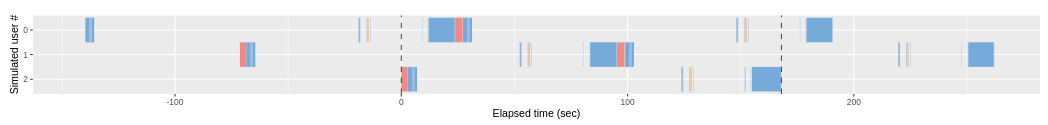
\includegraphics[scale=.4]{paperWSCAD2021/figures/user_PI3_3_worker_edit.jpg}\\(c) 3 usuários
 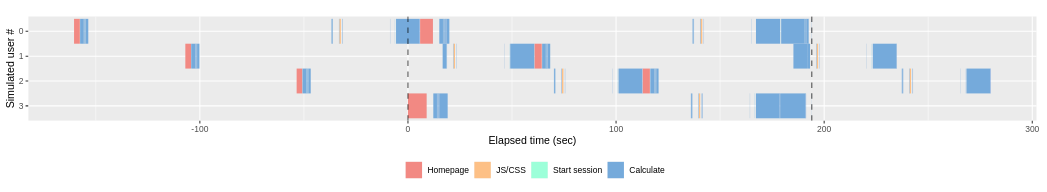
\includegraphics[scale=.4]{paperWSCAD2021/figures/user_PI3_4_worker.png}\\(d) 4 usuários
\caption{Traço de execução do simulador na Raspberry PI3.}
  \label{fig:PI3}
\end{figure}

\section{Conclusão} \label{sec:conlusao}
O experimento conduzido permitiu concluir que a Raspberry Pi 3 atende como suporte de \emph{hardware} o serviço especificado para o WebSYHDA quando existe um baixo número de usuários simultâneos. Seu uso em produção, portanto, seria inviável, embora este hardware possa ser considerado como plataforma de desenvolvimento ou em uso de pequenos laboratórios.  Por sua vez, a arquitetura x86 apresentou, em termos de escalabilidade, um desempenho adequado para um número que pode ser considerado médio de usuários simultâneos. 

Com tais dados, pudemos demonstrar a capacidade da Raspberry Pi 3 em atender a aplicação de forma pessoal, ou seja, um atendimento interno a poucos usuários simultâneos. Demonstrando também a viabilidade de atendimento a um número maior de usuários, dado a ociosidade do \emph{hardware} quando já alcançado o limite indicado pelo simulador.

Com isso, como trabalhos futuros, pretende-se fazer uso de técnicas de \emph{tuning} para um novo teste de melhor aproveitamento da Raspberry Pi 3. Também pretende-se propor a recodificação da aplicação utilizando o modelo de arquitetura de micro serviços, dado sua orquestração permitida assim conseguindo escalonar de melhor forma, acredita-se conseguir, assim, extrair o máximo que o \emph{hardware} tem a oferecer sem a necessidade de reduzir a aplicação. 


\bibliographystyle{sbc}
\bibliography{sbc-template}
\label{fimdotexto}

\end{document}
